
\chapter*{Jawaban untuk Latihan Terpilih}

\section*{Bagian \ref{sec:Accuracy}}

\addcontentsline{toc}{chapter}{Jawaban untuk Latihan Terpilih}
\fancyhead[RE]{Jawaban untuk Latihan Terpilih}
\fancyhead[LO]{}
\begin{description}
\item [{\ref{exc:abserr14}:}] $0.83333$
\item [{\ref{exc:abserr7}:}] $.2353263818643$ dan $.2343263818643$
\item [{\ref{exc:abserr18}a:}] $.2349438537911$ dan $.2347090273506$
\item [{\ref{exc:abserr8}:}] $(p,\tilde{p})\in\left\{ \left(\frac{1}{3},\frac{97}{300}\right),\ \left(\frac{1}{3},\frac{103}{300}\right),\ \left(-\frac{1}{3},-\frac{97}{300}\right),\ \left(-\frac{1}{3},-\frac{103}{300}\right)\right\} $
\item [{\ref{exc:abserr9}:}] $p=\pm1$ dan $\tilde{p}$ dapat berupa apa
pun; atau $p=\tilde{p}\neq0$.
\item [{\ref{exc:abserr10}:}] (i) $8.99999974990351$ (ii) $2.5009649(10)^{-7}$
(iii) $2.7788499(10)^{-8}$ (iv) $(10)^{-14}$ (v) $2.5009647(10)^{-7}$
\end{description}

\section*{Bagian \ref{sec:Taylor}}
\begin{description}
\item [{\ref{exc:taylor3}:}] $T_{3}(x)=x^{2}$. $R_{3}(x)=\frac{\xi\sin(\xi)-4\cos(\xi)}{24}x^{4}$.
\item [{\ref{exc:taylor9}:}] $10.760$
\item [{\ref{exc:taylor7}:}] $\xi(\pi)=\cos^{-1}\left(\frac{12\pi^{2}-48}{\pi^{4}}\right)\approx0.7625$.
\end{description}

\section*{Bagian \ref{sec:Speed}}
\begin{description}
\item [{\ref{exc:convergence-2}:}] $\alpha=1$
\item [{\ref{exc:convergence-6}:}] $O\left(\frac{1}{n}\right)$
\item [{\ref{exc:convergence-7}:}] $O\left(\frac{1}{\sqrt{n}}\right)$
\item [{\ref{exc:convergence-9}:}] $O\left(\frac{1}{n}\right)$
\item [{\ref{exc:convergence-13}:}] 4 iterasi
\end{description}

\section*{Bagian \ref{sec:Recursion}}
\begin{description}
\item [{\ref{exc:recursion}:}] (a) 1 lebih banyak daripada 4 kali jumlah
yang diperlukan untuk kisi $2^{n-1}\times2^{n-1}$. (b) 0 (c) 0
\item [{\ref{exc:recursion-7}:}] (a) $S(n-1,k-1)$ (b) $k\cdot S(n-1,k)$
\end{description}

\section*{Bagian \ref{sec:Bisection}}
\begin{description}
\item [{\ref{exc:bisection3}c:}] Dalam 27 iterasi, kita memperoleh $0.666666664928$,
yang berjarak kurang dari $10^{-8}$ dari suatu akar sebenarnya.
\item [{\ref{exc:bisection3}f:}] Dalam 27 iterasi, kita memperoleh $21.9911485687$,
yang berjarak kurang dari $10^{-8}$ dari suatu akar sebenarnya.
\item [{\ref{exc:bisection}:}] (a) $0.625$ (b) $1.09375$
\item [{\ref{exc:bisection-2}:}] $\frac{37\pi}{2}$
\item [{\ref{exc:bisection-3}:}] 33
\item [{\ref{exc:bisection-5}:}] Salah satu kemungkinan isi berkas\texttt{
collatz.m} adalah \begin{verbatim}
%%%%%%%%%%%%%%%%%%%%%%%%%%%%%%%%%%%%%%%%%%%%%%%%%%%
% Written by       on                             %
% Purpose: implementation of the collatz function %
% INPUT: integer n                                %
% OUTPUT: n/2 or 3n+1 depending on whether n is   %
%        even or odd                              %
%%%%%%%%%%%%%%%%%%%%%%%%%%%%%%%%%%%%%%%%%%%%%%%%%%%
function res=collatz(n)
  if (ceil(n/2)==n/2)
    res=n/2
  else
    res=3*n+1
  end%if
end%function
\end{verbatim}
\item [{\ref{exc:bisection-6}:}] (a) $\sqrt{20\pi}$
\end{description}

\section*{Bagian \ref{sec:Fixedpt}}
\begin{description}
\item [{\ref{exc:fixedpt-16}:}] (i) Hipotesis teorema nilai rata-rata
terpenuhi. (ii) $c\approx\text{\textminus}2.540793513382845$.
\item [{\ref{exc:fixedpt-2}:}] (i) Hipotesis teorema nilai rata-rata tidak
terpenuhi.
\item [{\ref{exc:fixedpt-3}:}] (i) Hipotesis teorema nilai rata-rata terpenuhi.
(ii) $c\approx17.41987374102208$.
\item [{\ref{exc:fixedpt-4}:}] $-2$ dan $5$
\item [{\ref{exc:fixedpt-5}:}] $-1$ dan $-\frac{1}{3}$
\item [{\ref{exc:fixedpt-7}:}] $f_{1}(x)=\sqrt[5]{\frac{4-6x^{2}}{3}}$
dan $f_{2}(x)=\sqrt{\frac{4-3x^{5}}{6}}$. Masih ada banyak kemungkinan
lain.
\item [{\ref{exc:fixedpt-9}:}] $f_{1}(x)=\frac{-(x^{2}-5x+1)(\log_{2}3)-x^{2}-1}{5}$
dan $f_{2}(x)=\sqrt{-(\log_{2}3)(x^{2}-5x+1)-5x-1}$. Masih ada banyak
kemungkinan lain.
\item [{\ref{exc:fixedpt-11}:}] 1.326008542399018, 1.598751095046933,
1.737721941251104, 1.779703798972744, 1.788512049183622; barisan ini
tampaknya konvergen.
\item [{\ref{enu:usingOctave}c:}] 1.79047660196506
\item [{\ref{enu:usingWeb}c:}] Diagram jaring pada $[.8,2]$ adalah:

\begin{center}
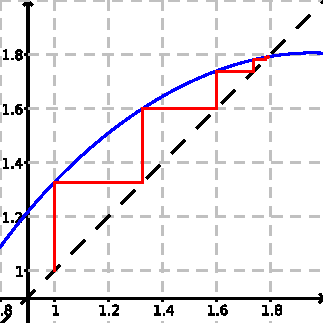
\includegraphics{figures/roots-fixedpt20}
\par\end{center}
\item [{\ref{exc:fixedpt-14}:}] (a) 15 (b) Persamaan $g(x)=x$ dan $f(x)=x$
ekuivalen.
\item [{\ref{exc:fixedpt-15}:}] $-\frac{1}{4}$
\end{description}

\section*{Bagian \ref{sec:fixedptOrder}}
\begin{description}
\item [{\ref{exc:orderOfConvergence-2}:}] (a) 15. PETUNJUK: Turunan boleh
dibatasi pada interval $[1.618033988749895,2.5]$ alih-alih seluruh
interval $[.5,3.5]$. Mengapa? Di sisi lain, jika seluruh interval
$[.5,3.5]$ juga dipertimbangkan, diperoleh batas sebesar 43. (b)
Sebenarnya diperlukan 15 iterasi.
\item [{\ref{exc:orderOfConvergence-4}:}] $a_{1}\approx1.942415717$ dan
$a_{2}\approx1.623271404$
\item [{\ref{exc:orderOfConvergence-5}:}] $2.732050809$. PETUNJUK: gunakan
$f(x)=\sqrt[4]{2x^{3}+4x^{2}-4x-4}$. Mengapa?
\item [{\ref{enu:aitkensOnSequence}:}] $a_{0}=3$, $a_{1}=\frac{3}{2}$,
dan $a_{2}=\frac{4}{3}$
\item [{\ref{exc:orderOfConvergence-7}:}] Ya. Metode delta-kuadrat Aitken
dirancang untuk mempercepat kekonvergenan barisan yang konvergen secara
linear, dan $\langle a_{n}\rangle$ merupakan barisan yang konvergen
secara linear.
\item [{\ref{exc:orderOfConvergence-9}:}] $a_{1}\approx2.152904629$ dan
$a_{2}\approx1.873464044$
\item [{\ref{exc:orderOfConvergence-10}:}] $\frac{3}{2}$ atau $0$
\item [{\ref{Steffensens}:}] $\hat{x}\approx5.259185715$
\end{description}

\section*{Bagian \ref{sec:newtonsMethod}}
\begin{description}
\item [{\ref{newton-1}c:}] Dengan menggunakan $x_{0}=2.5$, kita memperoleh
$x_{6}=1.47883214733021$.
\item [{\ref{newton-1}d:}] Dengan menggunakan $x_{0}=3.5$, kita memperoleh
$x_{7}=0.948434069919634$.
\item [{\ref{secant}c:}] Dengan menggunakan $x_{0}=2$ dan $x_{1}=3$,
kita memperoleh $x_{8}=1.47883214766643$.
\item [{\ref{secant}d:}] Dengan menggunakan $x_{0}=3$ dan $x_{1}=4$,
kita memperoleh $x_{10}=0.948434069243393$.
\item [{\ref{exc:newton}c:}] Dengan menggunakan $x_{0}=2.5$, kita memperoleh
$x_{18}=0.948434068437721$.
\item [{\ref{exc:newton}d:}] Dengan menggunakan $x_{0}=3.5$, kita memperoleh
$x_{15}=0.948434069313413$.
\item [{\ref{exc:newton-1}c:}] Dengan menggunakan $x_{0}=2$ dan $x_{1}=3$,
kita memperoleh $x_{10}=1.47883214733021$. Selisih antara $x_{10}$
dan $x_{8}$ kira-kira $3.3(10)^{-10}$, sehingga $x_{8}$ memang
akurat hingga $10^{-5}$.
\item [{\ref{exc:newton-1}d:}] Dengan menggunakan $x_{0}=3$ dan $x_{1}=4$,
kita memperoleh $x_{12}=0.948434069919636$. Selisih antara $x_{12}$
dan $x_{10}$ kira-kira $6.7(10)^{-10}$, sehingga $x_{10}$ memang
akurat hingga $10^{-5}$.
\item [{\ref{newton1}b:}] $x_{14}=0.580055888962675$.
\item [{\ref{exc:newton-4}b:}] Pada soal \ref{newton1}, $x_{14}=0.580055888962675$.
Dalam soal ini, $x_{14}=0$. Mengapa?
\item [{\ref{exc:newton-5}:}] $x_{10}=3.739599358563032$.
\item [{\ref{exc:newton-7}:}] Diperlukan 16 iterasi untuk mencapai toleransi
$0.0002$ ($|x_{15}-x_{14}|\approx0.000275$ dan $|x_{16}-x_{15}|\approx0.000184$).
$x_{12}=-0.181396689151049$, $x_{13}=-0.182015461369422$, $x_{14}=-0.182428614744863$,
$x_{15}=-0.182704334912558$, dan $x_{16}=-0.182888275080047$. $a_{12}=-0.183258770722810$,
$a_{13}=-0.183257488055966$ dan $a_{14}=-0.183256917323895$. Karena
akar eksak hingga 15 tempat desimal adalah $p\approx-0.183256460290832$,
kita melihat bahwa metode delta-kuadrat Aitken mempercepat kekonvergenan
dalam arti bahwa $a_{n}$ lebih dekat ke limit daripada $x_{n}$ (sebagaimana
ditunjukkan untuk $n=12,13,14$, dan seperti yang diharapkan untuk
metode delta-kuadrat Aitken yang diterapkan pada barisan yang konvergen
secara linear). Namun, orde kekonvergenannya tidak meningkat. Barisan
$\langle a_{n}\rangle$ masih konvergen secara linear. 
\begin{align*}
\frac{|a_{12}-p|}{|a_{13}-p|} & \approx2.2480\\
\frac{|a_{13}-p|}{|a_{14}-p|} & \approx2.2487
\end{align*}
misalnya, merupakan bukti bahwa $\lim_{n\to\infty}\frac{|a_{n+1}-p|}{|a_{n}-p|^{1}}=\lambda$
untuk suatu $\lambda\approx2.25$.
\item [{\ref{exc:newton-9}:}] (a) $\pi$ (b) Metode Newton akan gagal
karena $g'(0)=0$. (c) 6 (d) $-4.4$ atau $-4.3$.
\item [{\ref{exc:newton-10}c:}] Dalam 18 iterasi, kita memperoleh $0.666666668082383$,
yang berjarak kurang dari $10^{-8}$ dari suatu akar sebenarnya. Ini
adalah akar yang sama dengan yang ditemukan oleh metode bagi dua,
tetapi metode bagi dua memerlukan waktu lebih lama, yaitu 27 iterasi.
\item [{\ref{exc:newton-10}f:}] Dalam 9 iterasi, kita memperoleh $21.9911485743912$,
yang berjarak kurang dari $10^{-8}$ dari suatu akar sebenarnya. Ini
adalah akar yang sama dengan yang ditemukan oleh metode bagi dua,
tetapi metode bagi dua memerlukan waktu lebih lama, yaitu 27 iterasi.
\item [{\ref{exc:newton-13}:}] $3.555963292212723$
\end{description}

\section*{Bagian \ref{sec:moreConvergenceDiagrams}}
\begin{description}
\item [{\ref{exc:more-1}:}] $f$ dan (a), $g$ dan (d), $h$ dan (b),
$l$ dan (c)
\item [{\ref{exc:more-5}:}] $f$ dan (b), $g$ dan (c), $h$ dan (d),
$l$ dan (a)
\end{description}

\section*{Bagian \ref{sec:RootsOfPolynomials}}
\begin{description}
\item [{\ref{exc:polynomials-7}:}] $g(2)=5$ dan $g'(2)=-8$
\item [{\ref{exc:polynomials-10}b:}] $x_{1}=\frac{21}{8}$ dan $x_{2}=\frac{241003}{100544}$
\item [{\ref{exc:polynomials-14}:}] $-8,\ -2.33333,\ 0.33333,\ 2+i,\ 2-i$
\item [{\ref{exc:polynomials-17}:}] $-2,\ 0.76393,\ 5.23607,\ 0.66667+0.57735i,\ 0.66667-0.57735i$
\item [{\ref{exc:polynomials-18}b:}] Nilai-nilainya berubah, tetapi tidak
dalam lima tempat desimal pertama.
\item [{\ref{exc:polynomials-9}:}] (i) \texttt{-109.372462336481} (ii)
\texttt{-109.372462336481} (iii) \texttt{ans = 0}
\item [{\ref{exc:polynomials-11}:}] (i) \texttt{948.990683139955} (ii)
\texttt{948.990683139955} (iii) \texttt{ans = 1}
\item [{\ref{exc:polynomials-13}:}] $\ $\index{metode Horner!kode} \begin{verbatim}
%%%%%%%%%%%%%%%%%%%%%%%%%%%%%%%%%%%%%%%%%%%%%%%%%%%%
% Written by Dr. Len Brin          15 January 2014 %
% Purpose: Implementation of Newton's Method       %
%        for polynomials of the form               %
%   p(x) = c1 + c2*x + c3*x^2 + ... + c(n+1)*x^n   %
%        using Horner's Method, n > 1.             %
% INPUT: coefficients c; tolerance tol; maximum    %
%        number of iterations N                    %
% OUTPUT: approximations to all roots, roots       %
%%%%%%%%%%%%%%%%%%%%%%%%%%%%%%%%%%%%%%%%%%%%%%%%%%%%
function roots = newthornall(c,tol,N,x0)
  n=length(c)-1;
  for i=1:n-2
    res=newtonhorner(c,x0,tol,N)
    roots(i)=res;
    x0=roots(i);
    c=deflate(c,x0);
  end%for
  [roots(n-1),roots(n)]=quadraticRoots(c(3),c(2),c(1));
end%function
\end{verbatim}

\begin{description}
\item [{Catatan:}] Kode ini sering berhasil, tetapi dapat dengan mudah
tidak menghasilkan apa pun. Sebagai contoh,

\begin{center}
\texttt{newthornall({[}56,-152,140,-17,-48,9{]},1e-5,100,2)}
\par\end{center}

menghasilkan \begin{verbatim}
res =  0.763932022500484
res =  5.23606797749979
res = Method failed---maximum number of iterations reached
error: newthornall: A(I) = X: X must have the same size as I
error: called from:
error:   .../newthornall.m at line 16, column 13
\end{verbatim}

Kode ini gagal menemukan akar riil ketiga, $-2$. Setelah menemukan
dua akar pertama, diperoleh polinom hasil deflasi berikut:
\[
\begin{gathered}14.00000000000065-16.99999999999987x+\qquad\\
\qquad6.00000000000002x^{2}+9.00000000000000x^{3}.
\end{gathered}
\]
Dengan polinom kubik ini dan nilai awal $5.23606797749979$, metode
Newton tidak konvergen ke $-2$. Di sisi lain, \texttt{newthornall({[}56,-152,140,-17,-48,9{]},1e-5,100,-2)}
menghasilkan \begin{verbatim}
res = -2
res =  0.763932022500211
res =  5.23606797749979
ans =

 Columns 1 and 2:

  -2.000000000000000 + 0.000000000000000i   0.763932022500211 + 0.000000000000000i

 Columns 3 and 4:

   5.236067977499789 + 0.000000000000000i   0.666666666666667 + 0.577350269189623i

 Column 5:

   0.666666666666667 - 0.577350269189623i
\end{verbatim}

Setelah terlebih dahulu menemukan $-2$, kode ini tidak mengalami
masalah dalam menemukan akar-akar lainnya.
\end{description}
\item [{\ref{exc:polynomials-15}:}] (a) 
\[
\begin{gathered}1.5858\\
-13\\
4.4142\\
-2+2.2361i\\
-2-2.2361i
\end{gathered}
\]
(b) 
\[
\begin{gathered}3-1.4142i\\
-2.6\\
-2+2.2361i\\
-2-2.2361i\\
3+1.4142i
\end{gathered}
\]
\end{description}

\section*{Bagian \ref{sec:RootsBracketing}}
\begin{description}
\item [{\ref{exc:bracketing}:}] (a) $x_{4}=2.1806$ (e) $x_{10}=-502.19$
(j) $x_{3}=1.0079$
\item [{\ref{exc:bracketing-1}:}] (a) $x_{5}=2.1798$ (e) $x_{9}=-502.19$
(j) $x_{6}=1.0079$
\item [{\ref{exc:bracketing-2}:}] (a) $x_{7}=2.1798$ (e) $x_{6}=-499.98$
(j) $x_{5}=1.0080$
\item [{\ref{exc:bracketing-3}:}] (a) $x_{7}=2.1798$ (e) $x_{2}=-499.98$
(j) $x_{3}=4.1495$
\item [{\ref{exc:bracketing-4}:}] (a) $x_{9}=2.17975713685875$ (e) $x_{18}=-502.188059117229$
(j) $x_{4}=1.00794427892360$
\item [{\ref{exc:bracketing-5}:}] (a) $x_{6}=2.17975706647997$ (e) $x_{10}=-502.188059235320$
(j) $x_{8}=1.00794427848101$
\item [{\ref{exc:bracketing-6}:}] (a) $x_{6}=2.17975706647996$ (e) $x_{9}=-502.188059235320$
(j) $x_{4}=1.00794427848094$
\item [{\ref{exc:bracketing-7}:}] (a), (e), dan (j): Interpolasi kuadratik
invers terkurung tidak lebih lambat daripada metode posisi palsu atau
metode Newton terkurung.
\item [{\ref{exc:bracketing-8}:}] \index{metode Steffensen!kode} \texttt{bracketedSteffensens.m}
dapat diunduh dari \href{http://lqbrin.github.io/tea-time-numerical/ancillaries.html}{situs pendamping}.
\begin{verbatim}
%%%%%%%%%%%%%%%%%%%%%%%%%%%%%%%%%%%%%%%%%%%%%%%%%%%
% Written by Dr. Len Brin         15 January 2014 %
% Purpose: Implementation of Steffensen's method  %
% INPUT: function f; initial value x0; tolerance  %
%        TOL; maximum iterations N0               %
% OUTPUT: approximation x and number of           %
%        iterations i; or message of failure      %
%%%%%%%%%%%%%%%%%%%%%%%%%%%%%%%%%%%%%%%%%%%%%%%%%%%
function [x,i] = bracketedSteffensens(f,a,b,TOL,N0)
  i=1;
  A=f(a);
  B=f(b);
  while (i<=N0)
    b
    x0=b;
    x1=B;
    x2=f(x1);
    if (abs(x2-x1)<TOL)
      x=x2;
      disp(" ");
      return
    end%if
    x=x0-(x1-x0)^2/(x2-2*x1+x0);
    if (x<min([a,b]) || x>max([a,b]))
      x=a+(b-a)/2;
    end%if
    if (abs(x-x2)<TOL)
      disp(" ");
      return
    end%if
    X=f(x);
    if ((B<b && X>x) || (B>b && X<x))
      a=b; A=B;
    end%if
    b=x; B=X;
    i=i+1;
  end%while
  x="Method failed---maximum number of iterations reached";
end%function 
\end{verbatim}
\item [{\ref{exc:bracketing-9}:}] (a) $x_{6}=2.17975706643814$ (e) $x_{11}=-502.188059386686$
(j) $x_{9}=1.00794427672537$
\item [{\ref{exc:bracketing-13}:}] (a), (e), dan (j): Jika hanya menghitung
jumlah iterasi, interpolasi kuadratik invers terkurung tidak lebih
lambat daripada metode Steffensen dengan pengurungan. Namun, metode
Steffensen dengan pengurungan memerlukan dua penghitungan nilai fungsi
per iterasi, sehingga dalam praktiknya memerlukan daya komputasi lebih
dari dua kali lipat dibandingkan interpolasi kuadratik invers terkurung.
\item [{\ref{exc:bracketing-11}:}] (a) $x_{6}=2.17975706647996$ (e) $x_{8}=-502.188059227438$
(j) $x_{4}=1.00794427848094$
\item [{\ref{exc:bracketing-14}:}] (a) dan (j): Karena akar bernilai sekitar
$1$, tidak ada perbedaan antara pengujian galat absolut dan galat
relatif. (e) Karena akar bernilai sekitar lima ratus, metode berhenti
ketika galat absolut baru sekitar $10^{-6}\cdot500=5(10)^{-4}$. Akibatnya,
metode berhenti satu iterasi lebih awal ketika memeriksa galat relatif
dibandingkan ketika memeriksa galat absolut.
\end{description}

\section*{Bagian \ref{sec:polynomialLagrange}}
\begin{description}
\item [{\ref{exc:interpolation-lagrange-5}:}] $4$
\item [{\ref{exc:interpolation-lagrange-14}:}] $3$, $\frac{18+\sqrt{142}}{7}$,
atau $\frac{18-\sqrt{142}}{7}$
\item [{\ref{exc:interpolation-lagrange-15}:}] $8$
\end{description}

\section*{Bagian \ref{sec:polynomialNewton}}
\begin{description}
\item [{\ref{exc:interpolation-newton-5}:}] $P_{2}(x)=-0.001642458785316x^{2}+1.64927376355948x+10$
\item [{\ref{exc:interpolation-newton-6}:}] $P_{3}(x)=2x-1$. Apakah derajat
$1$ sesuai dengan yang Anda harapkan?
\item [{\ref{exc:interpolation-newton-9}:}] (a) $\frac{3}{40000}f^{(4)}(\xi_{8.4})$
(b) $8.7364(10)^{-5}{\displaystyle \max_{x\in[8.1,8.7]}}\left|f^{(4)}(x)\right|$
(c) $.52501$ 
\item [{\ref{exc:interpolation-newton-10}:}] $0.5x^{3}+1.5x^{2}+0.335x+0.951$
\item [{\ref{exc:interpolation-newton-13}:}] $f$ dan (b), $g$ dan (c),
$h$ dan (d), $l$ dan (a)
\end{description}

\section*{Bagian \ref{sec:NumericalRudiments}}
\begin{description}
\item [{\ref{exc:rudiments-4}c:}] $f'\left(x_{0}+\frac{h}{2}\right)\approx\frac{f(x_{0}+h)-f(x_{0})}{h}$
\item [{\ref{exc:rudiments-5}c:}] $f'\left(x_{0}+\frac{h}{2}\right)\approx\frac{f(x_{0}+h)-f(x_{0})}{h}$
\item [{\ref{exc:rudiments-1}:}] (a) $20.32712878304436$ (e) $0.6321205268681437$
(g) $0.2325441461772505$
\item [{\ref{exc:rudiments-11}:}] (a) (i) $e^{3}-e^{-4}$ (ii) $0.2599074987454273$
(e) (i) $1-e^{-1}$ (ii) $3.196041398201288(10)^{-8}$\\
(g) (i) $\ln2$ (ii) $1.2110575916990385(10)^{-5}$
\item [{\ref{exc:rudiments-12}:}] $1.19336533331362$
\item [{\ref{exc:rudiments-13}b:}] $.19336533331362$
\item [{\ref{exc:rudiments-14}:}] $35$
\item [{\ref{exc:rudiments-16}:}] $\frac{28}{15}$
\item [{\ref{exc:rudiments-17}:}] $-1$
\item [{\ref{exc:rudiments-18}:}] $-23$
\item [{\ref{exc:rudiments-20}:}] $f'(x_{0}+3h)\approx\frac{7f(x_{0}+2h)-15f(x_{0})+8f(x_{0}-h)}{6h}$
\item [{\ref{exc:rudiments-22}:}] $f'(x_{0}-h)\approx\frac{-f(x_{0}+2h)+9f(x_{0})-8f(x_{0}-h)}{6h}$
\item [{\ref{exc:rudiments-23}:}] $f'(x_{0})\approx\frac{-f(x_{0}+3h)+9f(x_{0}+h)-8f(x_{0})}{6h}$
\item [{\ref{exc:rudiments-24}:}] $\int_{x_{0}+\theta_{0}h}^{x_{0}+\theta_{1}h}f(x)dx\approx-\frac{h}{2}\cdot\frac{\theta_{1}-\theta_{0}}{\theta_{3}-\theta_{2}}\left((2\theta_{2}-\theta_{1}-\theta_{0})f(x_{0}+\theta_{3}h)-(2\theta_{3}-\theta_{1}-\theta_{0})f(x_{0}+\theta_{2}h)\right)$
\item [{\ref{exc:rudiments-25}:}] $\int_{x_{0}}^{x_{0}+2h}f(x)dx\approx\frac{h}{2}\left[f(x_{0})+3f\left(x_{0}+\frac{4}{3}h\right)\right]$
\item [{\ref{exc:rudiments-27}:}] $\int_{x_{0}}^{x_{0}+h}f(x)dx\approx\frac{h}{2}\left[f(x_{0})+f(x_{0}+h)\right]$
\end{description}

\section*{Bagian \ref{sec:UndeterminedCoefficients}}
\begin{description}
\item [{\ref{exc:undetermined}:}] (b) ${\displaystyle f'\left(x_{0}+\frac{h}{4}\right)\approx\frac{f(x_{0}+h)-f(x_{0})}{h}}$\\
(f) ${\displaystyle f'\left(x_{0}-h\right)\approx\frac{-3f(x_{0}-h)+4f(x_{0})-f(x_{0}+h)}{2h}}$\\
(h) ${\displaystyle f'\left(x_{0}-h\right)\approx\frac{-7f(x_{0}-h)+16f(x_{0}+2h)-9f(x_{0}+3h)}{12h}}$\\
(l) ${\displaystyle f'\left(x_{0}\right)\approx\frac{-3f(x_{0}-h)-10f(x_{0})+18f(x_{0}+h)-6f(x_{0}+2h)+f(x_{0}+3h)}{12h}}$
\item [{\ref{exc:undetermined-1}:}] (b) ${\displaystyle f''\left(x_{0}-h\right)\approx\frac{f(x_{0}-h)-2f(x_{0})+f(x_{0}+h)}{h^{2}}}$\\
(d) ${\displaystyle f''\left(x_{0}-h\right)\approx\frac{f(x_{0}-h)-4f(x_{0}+2h)+3f(x_{0}+3h)}{6h^{2}}}$\\
(h) ${\displaystyle f''\left(x_{0}\right)\approx\frac{11f(x_{0}-h)-20f(x_{0})+6f(x_{0}+h)+4f(x_{0}+2h)-f(x_{0}+3h)}{12h^{2}}}$
\item [{\ref{exc:undetermined-2}:}] (d) ${\displaystyle \int_{x_{0}}^{x_{0}+h}f(x)dx\approx hf(x_{0})}$\\
(f) ${\displaystyle \int_{x_{0}}^{x_{0}+2h}f(x)dx\approx h\left(f\left(x_{0}+\frac{2}{3}h\right)+f\left(x_{0}+\frac{4}{3}h\right)\right)}$\\
(h) ${\displaystyle \int_{x_{0}}^{x_{0}+h}f(x)dx\approx\frac{h}{2}\left(f(x_{0})+f(x_{0}+h)\right)}$\\
(j) ${\displaystyle \int_{x_{0}}^{x_{0}+2h}f(x)dx\approx\frac{h}{2}\left(3f\left(x_{0}+\frac{2}{3}h\right)+f(x_{0}+2h)\right)}$
\end{description}

\section*{Bagian \ref{sec:calculusErrorAnalysis}}
\begin{description}
\item [{\ref{exc:calculusErrors-4}:}] $f'(-2.7)\approx-0.9151775$; $f'(-2.5)\approx1.5014075$;
$f'(-2.3)\approx2.17825$; $f'(-2.1)\approx1.11535$
\item [{\ref{exc:calculusErrors-6}:}] $0.4897985468241977$
\item [{\ref{exc:calculusErrors-7}:}] $149/24=6.208\overline{3}$
\item [{\ref{exc:calculusErrors-1}:}] (c) $0.4693956404725931$ (e) $17/2=8.5$
\item [{\ref{exc:calculusErrors-2}:}] (c) $0.5$ (e) $81/16=5.0625$
\item [{\ref{exc:calculusErrors-37}:}] (c) $8.57775220962087(10)^{-5}$
(e) $0.008\overline{3}$
\item [{\ref{exc:calculusErrors-38}:}] (c) $0.02031712882950837$ (e)
$2.3$
\item [{\ref{exc:calculusErrors-39}:}] (c) $0.0102872306978985$ (e) $1.1375$
\item [{\ref{exc:calculusErrors-19}:}] $0$
\item [{\ref{exc:calculusErrors-20}:}] $288666.8155482048$
\item [{\ref{exc:calculusErrors-8}b:}] batas bawah: $1565.147456974753$
batas atas: $2334.925631788689$ nilai sebenarnya: $1915.502415038936$
\item [{\ref{exc:calculusErrors-9}b:}] $3.142092629759007$
\item [{\ref{exc:calculusErrors-21}:}] suku galat: $O(h^{2}f'(\xi))$
derajat ketelitian: $0$
\item [{\ref{exc:calculusErrors-22}:}] suku galat: $O(h^{4}f'''(\xi))$
derajat ketelitian: $2$
\item [{\ref{exc:calculusErrors-23}:}] suku galat: $O(h^{4}f'''(\xi))$
derajat ketelitian: $2$
\item [{\ref{exc:calculusErrors-24}:}] suku galat: $O(h^{5}f^{(4)}(\xi))$
derajat ketelitian: $3$
\item [{\ref{exc:calculusErrors-25}:}] $O(hf''(\xi))$
\item [{\ref{exc:calculusErrors-26}:}] $O(h^{4}f^{(5)}(\xi))$
\item [{\ref{exc:calculusErrors-27}:}] $O(hf'''(\xi))$
\item [{\ref{exc:calculusErrors-28}:}] $O(h^{3}f^{(5)}(\xi))$
\item [{\ref{exc:calculusErrors-29}:}] $0.0134k$ untuk suatu konstanta
$k$ yang bergantung pada rumus hampiran, bukan pada fungsi $\sin x$.
\item [{\ref{exc:calculusErrors-30}:}] (a) $O(h^{3})$ (b) $1$ (c) $\frac{\sqrt{3}}{2}\pi\approx2.720699046351327$
(d) $\frac{\pi^{3}}{36}\approx0.8612854633416616$ (e) galat absolut
sebenarnya: $0.7206990463513265$
\item [{\ref{exc:calculusErrors-31}:}] $-\frac{1}{2}$
\item [{\ref{exc:calculusErrors-32}:}] $O(h^{2})$
\item [{\ref{exc:calculusErrors-33}:}] $0$
\item [{\ref{exc:calculusErrors-40}:}] $10506.03569166666$
\item [{\ref{exc:calculusErrors-34}:}] hampiran 1: $\frac{-3(1.22140)+4(1.10517)-1}{-.2}=1.2176$;
hampiran 2: $\frac{1.34986-1.10517}{.2}=1.22345$; hampiran 3: $\frac{-3(1.22140)+4(1.34986)-1.49182}{.2}=1.2171$;
peringkat: 3,1,2; Jawaban lain dapat diterima.
\item [{\ref{exc:calculusErrors-35}:}] $2.58629507364657$; $h=.0000474853515625$
\end{description}

\section*{Bagian \ref{sec:Composite}}
\begin{description}
\item [{\ref{exc:calculus-composite}:}] (c) $17.52961733248352$ (e) $1.560867019857898$
\item [{\ref{exc:calculus-composite-7}:}] (c) $19.3773960369059$ (e)
$1.569045013890161$
\item [{\ref{exc:calculus-composite-8}:}] (c) $18.14554356729098$ (e)
$1.563593017868653$
\item [{\ref{exc:calculus-composite-9}:}] (c) $18.14441877898906$ (e)
$1.563592239944993$
\item [{\ref{exc:calculus-composite-10}:}] (c) $17.73342635968343$ (e)
$1.561774648629937$
\item [{\ref{exc:calculus-composite-14}:}] 141
\item [{\ref{exc:calculus-composite-15}:}] 
\[
\int_{x_{0}}^{x_{0}+2h}f(x)dx\approx\frac{h}{3n}\left[f(x_{0})+f(x_{0}+2h)+2\sum_{i=1}^{n-1}f\left(x_{0}+2i\frac{h}{n}\right)+4\sum_{i=1}^{n}f\left(x_{0}+\left(2i-1\right)\frac{h}{n}\right)\right]
\]
\item [{\ref{exc:calculus-composite-16}:}] 
\begin{eqnarray*}
\int_{x_{0}}^{x_{0}+3h}f(x)dx & \approx & \frac{3h}{8n}\left[f(x_{0})+f(x_{0}+3h)+2\sum_{i=1}^{n-1}f\left(x_{0}+3i\frac{h}{n}\right)\right.\\
 &  & \qquad\left.+3\sum_{i=1}^{n}\left(f\left(x_{0}+\left(3i-2\right)\frac{h}{n}\right)+f\left(x_{0}+\left(3i-1\right)\frac{h}{n}\right)\right)\right]
\end{eqnarray*}
\item [{\ref{exc:calculus-composite-18}:}] $0.386259562814567$
\item [{\ref{exc:calculus-composite-1}:}] (a) $1.386294361119891$ (b)
$132$
\item [{\ref{exc:calculus-composite-19}:}] $3.109198655184147$; ya
\item [{\ref{exc:calculus-composite-20}:}] $0.3862939349171364$; 5
\item [{\ref{exc:calculus-composite-5}:}] Implementasi langsung, \texttt{adaptSimp()}:\index{Aturan Simpson adaptif!kode}

\begin{verbatim}
####################################################
# Written by Leon Brin                15 May 2014  #
# Purpose: Implementation of adaptive Simpson's    #
# rule                                             #
# INPUT: function f, interval endpoints a and b,   #
#        desired accuracy TOL.                     #
# OUTPUT: approximate integral of f(x) from a to b #
#         within TOL of actual.                    #
####################################################

function res = adaptSimp(f,a,b,TOL)
  h = (b-a)/4;
  f0 = f(a);
  f1 = f(a+h);
  f2 = f(a+2*h);
  f3 = f(a+3*h);
  f4 = f(b);
  error = abs(h*(f0-4*(f1+f3)+6*f2+f4))/45;
  if (error <= TOL)
    res = h/3*(f0+4*(f1+f3)+2*f2+f4);
  else
    res = adaptSimp(f,a,a+2*h,TOL/2) + adaptSimp(f,a+2*h,b,TOL/2);
  endif
endfunction
\end{verbatim}

Sepasang fungsi yang meminimalkan jumlah penghitungan nilai $f$,
\texttt{aSimp()} dan \texttt{adaptiveSimpsons()}:\begin{verbatim}
####################################################
# Written by Leon Brin                15 May 2014  #
# Purpose: Wrapper for aSimp()                     #
# INPUT: function f, interval endpoints a and b,   #
#        desired accuracy TOL.                     #
# OUTPUT: approximate integral of f(x) from a to b #
#         within TOL of actual.                    #
####################################################
function res = adaptiveSimpsons(f,a,b,TOL)
  res = aSimp(f,a,b,f(a),f((a+b)/2),f(b),TOL);
end#function

####################################################
# Written by Leon Brin                15 May 2014  #
# Purpose: Implementation of adaptive Simpson's    #
# rule                                             #
# INPUT: function f, interval endpoints a and b,   #
#        f0=f(a), f2=f((a+b)/2), f4=f(b), desired  #
#        accuracy TOL.                             #
# OUTPUT: approximate integral of f(x) from a to b #
#         within TOL of actual.                    #
####################################################
function res = aSimp(f,a,b,f0,f2,f4,TOL)
  h = (b-a)/4;
  f1 = f(a+h);
  f3 = f(a+3*h);
  error = abs(h*(f0-4*(f1+f3)+6*f2+f4))/45;
  if (error <= TOL)
    res = h/3*(f0+4*(f1+f3)+2*f2+f4);
  else
    res = aSimp(f,a,a+2*h,f0,f1,f2,TOL/2) + aSimp(f,a+2*h,b,f2,f3,f4,TOL/2);
  end#if
end#function
\end{verbatim}

\textbf{CATATAN:} \texttt{aSimp()}, \texttt{adaptSimp()}, dan \texttt{adaptiveSimpsons()}
harus ditempatkan dalam berkas \texttt{.m} yang terpisah.\\
\texttt{adaptiveSimpsons()} adalah satu-satunya yang seharusnya digunakan
secara langsung. Fungsi lainnya dipanggil olehnya. Kode dapat diunduh
dari \href{http://lqbrin.github.io/tea-time-numerical/ancillaries.html}{situs pendamping}.
\item [{\ref{exc:calculus-composite-21}:}] \begin{verbatim}
>> f=@(x) log(sin(x));
>> adaptiveSimpsons(f,1,3,.002)
ans = -0.70293
\end{verbatim}
\item [{\ref{exc:calculus-composite-22}:}] (a) (i) \begin{verbatim}
>> format('long');
>> f=@(x) x*sin(x^2);
>> adaptiveSimpsons(f,0,2*pi,10^-5)
ans =  0.603500307287469
\end{verbatim}(ii) $ $ (iii) ya
\end{description}

\section*{Bagian \ref{sec:Extrapolation}}
\begin{description}
\item [{\ref{exc:calculus-extrapolation}:}] Jawaban akan bervariasi. Sebagai
contoh, dengan menggunakan $\alpha=\frac{1}{2}$, ${\displaystyle N_{1}(h)=\frac{8\sin^{-1}\left(1-\frac{h^{4}}{16}\right)-2\sin^{-1}\left(1-h^{4}\right)}{3}}$
memiliki galat $O(h^{6})$.
\item [{\ref{exc:calculus-extrapolation-1}:}] $O(h^{9})$
\item [{\ref{exc:calculus-extrapolation-2}:}] $\frac{16}{9}$
\item [{\ref{exc:calculus-extrapolation-3}:}] (a) $N(1.0)\approx0.4596976941318602$
dan $N(0.5)\approx0.489669752438509$\\
(b) (i) $N_{1}(1.0)\approx0.5196418107451577$ (ii) $N_{1}(1.0)\approx0.4996604385407252$\\
(c) asumsi (i), karena menghasilkan hampiran dengan galat sekitar
setengah dari galat $N(1.0)$, tepat seperti yang diharapkan jika
asumsi (i) benar.

\begin{description}
\item [{CATATAN:}] $\lim_{h\to0}\frac{1-\cos h}{h^{2}}=\frac{1}{2}$.
\end{description}
\item [{\ref{exc:calculus-extrapolation-7}:}] ${\displaystyle \frac{N(h)-12N(h/3)+27N(h/9)}{16}}$
\item [{\ref{exc:calculus-extrapolation-11}:}] (c) $18.1436194387278$
(e) $1.56359161739838$ (g) $3.10928992861842$
\item [{\ref{exc:calculus-extrapolation-8}:}] Kode berikut berfungsi,
tetapi tidak terlalu efisien dan bergantung pada fungsi compositeTrapezoidal()
yang berjalan dengan baik. Bahkan, inefisiensi tersebut disebabkan
oleh pemanggilan fungsi compositeTrapezoidal(). Setiap kali compositeTrapezoidal()
dipanggil, fungsi tersebut menghitung ulang nilai f yang telah dihitung
saat pemanggilan sebelumnya. Menghindari pengulangan pekerjaan ini
akan membuat rutin tersebut jauh lebih efisien. Dapatkah Anda memikirkan
cara untuk melakukannya? \texttt{romberg.m} dapat diunduh dari \href{http://lqbrin.github.io/tea-time-numerical/ancillaries.html}{situs pendamping}.
\index{integrasi Romberg!kode} \begin{verbatim}
####################################################
# Written by Dr. Len Brin              16 May 2014 #
# Purpose: Implementation of Romberg integration   #
# INPUT: function f, interval endpoints a and b,   #
#        tolerance tol                             #
# OUTPUT: approximate integral of f(x) from a to b #
####################################################
function integral = romberg(f,a,b,tol)
  N(1,1)=compositeTrapezoidal(f,a,b,1);
  N(2,1)=compositeTrapezoidal(f,a,b,2);
  N(2,2)=(4*N(2,1)-N(1,1))/3;
  i=2;
  while (abs(N(i,i)-N(i,i-1))>tol || abs(N(i,i)-N(i-1,i-1))>tol)
    i=i+1;
    N(i,1)=compositeTrapezoidal(f,a,b,2^(i-1));
    for j=2:i
      m=4^(j-1);
      N(i,j)=(m*N(i,j-1)-N(i-1,j-1))/(m-1);
    end#for
  end#while
  integral=N(i,i);
end#function
\end{verbatim}
\item [{\ref{exc:calculus-extrapolation-9}:}] (i) \begin{verbatim}
>> romberg(@(x) x*sin(x^2),0,2*pi,10^-5)
ans =  0.603500924593406
\end{verbatim}(ii) ${\displaystyle \left|\frac{1-\cos(4\pi^{2})}{2}-0.603500924593406\right|\approx2.34(10)^{-10}}$
(iii) ya, bahkan jauh melampaui syaratnya
\end{description}

\section*{Bagian \ref{sec:Splines}}
\begin{description}
\item [{\ref{exc:cubicSplines-8}:}] 
\[
S(x)=\begin{cases}
-.28+3.1861(x-.2)-3.208(x-.2)^{2}-10.693333(x-.2)^{3}, & x\in[.1,.2]\\
.0066+2.5465(x-.3)-3.188(x-.3)^{2}+.066667(x-.3)^{3}, & x\in[.2,.3]\\
.24+2.2277(x-.4)+10.626667(x-.4)^{3} & x\in[.3,.4]
\end{cases}
\]
\item [{\ref{exc:cubicSplines-12}:}] 
\[
S(x)=\begin{cases}
-.28+3.84613(x-.2)-20.0773(x-.2)^{2}-245.387(x-.2)^{3}, & x\in[.1,.2]\\
.0066+2.91347(x-.3)+10.7507(x-.3)^{2}+102.76(x-.3)^{3}, & x\in[.2,.3]\\
.24+0.1(x-.4)-38.8853(x-.4)^{2}-165.453(x-.4)^{3}, & x\in[.3,.4]
\end{cases}
\]
\item [{\ref{exc:cubicSplines-15}:}] \begin{verbatim}
>> [a,b,c,d]=naturalCubicSpline([.1,.2,.3,.4],[-.62,-.28,.0066,.24])
a =
  -0.2800000   0.0066000   0.2400000

b =
   3.1861   2.5465   2.2277

c =
  -3.20800  -3.18800   0.00000

d =
  -10.693333    0.066667   10.626667
\end{verbatim}
\item [{\ref{exc:cubicSplines-17}:}] \begin{verbatim}
>> [a,b,c,d]=clampedCubicSpline([.1,.2,.3,.4],[-.62,-.28,.0066,.24],0.5,0.1)
a =
  -0.2800000   0.0066000   0.2400000

b =
   3.84613   2.91347   0.10000

c =
  -20.077   10.751  -38.885

d =
  -245.39   102.76  -165.45
\end{verbatim}
\end{description}

\section*{Bagian \ref{sec:OdePendulum}}
\begin{description}
\item [{\ref{exc:odePendulum}:}] satu
\item [{\ref{exc:odePendulum-1}:}] dua
\item [{\ref{exc:odePendulum-3}:}] dua
\item [{\ref{exc:odePendulum-4}:}] $\dot{y}(t)=e^{t}$. Dengan menyubstitusikannya
ke $\dot{y}=y$ diperoleh $e^{t}=e^{t}$, suatu pernyataan yang benar.
\item [{\ref{exc:odePendulum-5}:}] $\ $ 
\begin{eqnarray*}
\dot{s}(t) & = & \frac{1}{2}e^{-t/2}\left(\sqrt{3}\cos\left(\frac{\sqrt{3}}{2}t\right)-\sin\left(\frac{\sqrt{3}}{2}t\right)\right)\\
\ddot{s}(t) & = & -\frac{1}{2}e^{-t/2}\left(\sqrt{3}\cos\left(\frac{\sqrt{3}}{2}t\right)+\sin\left(\frac{\sqrt{3}}{2}t\right)\right)
\end{eqnarray*}
 Dengan menyubstitusikannya ke $\ddot{s}+\dot{s}+s=0$ diperoleh 
\[
-\frac{1}{2}e^{-t/2}\left(\sqrt{3}\cos\left(\frac{\sqrt{3}}{2}t\right)+\sin\left(\frac{\sqrt{3}}{2}t\right)\right)+\frac{1}{2}e^{-t/2}\left(\sqrt{3}\cos\left(\frac{\sqrt{3}}{2}t\right)-\sin\left(\frac{\sqrt{3}}{2}t\right)\right)+e^{-t/2}\sin\left(\frac{\sqrt{3}}{2}t\right)=0,
\]
suatu pernyataan yang benar.
\item [{\ref{exc:odePendulum-7}:}] $\dot{r}(t)=\frac{1}{2\sqrt{t}}$ dan
$\ddot{r}(t)=-\frac{1}{4t\sqrt{t}}$. Dengan menyubstitusikannya ke
$\ddot{r}\dot{r}t^{2}=-\frac{1}{8}$ diperoleh $\left(-\frac{1}{4t\sqrt{t}}\right)\left(\frac{1}{2\sqrt{t}}\right)t^{2}=-\frac{1}{8}$,
suatu pernyataan yang benar untuk $t>0$.
\item [{\ref{exc:odePendulum-8}:}] $\dot{y}(t)=4e^{t}$. Dengan menyubstitusikannya
ke $\dot{y}=y$ diperoleh $4e^{t}=4e^{t}$, suatu pernyataan yang
benar. Selain itu, $y(0)=4e^{0}=4$ sebagaimana disyaratkan.
\item [{\ref{exc:odePendulum-9}:}] $\dot{s}(t)=-te^{-t^{2}}$. Dengan
menyubstitusikannya ke $\dot{s}=(1-2s)t$ diperoleh $-te^{-t^{2}}=\left(1-2\times\frac{1}{2}\left(1+e^{-t^{2}}\right)\right)t$,
suatu pernyataan yang benar. Selain itu, $s(0)=\frac{1}{2}(1+e^{0})=1$
sebagaimana disyaratkan.
\item [{\ref{exc:odePendulum-11}:}] $\dot{r}(t)=\frac{1}{2\sqrt{t}}$
dan $\ddot{r}(t)=-\frac{1}{4t\sqrt{t}}$. Dengan menyubstitusikannya
ke $\ddot{r}\dot{r}t^{2}=-\frac{1}{8}$ diperoleh $\left(-\frac{1}{4t\sqrt{t}}\right)\left(\frac{1}{2\sqrt{t}}\right)t^{2}=-\frac{1}{8}$,
suatu pernyataan yang benar untuk $t>0$. Selain itu, $r(9)=\sqrt{9}-3=0$
dan $\dot{r}(9)=\frac{1}{2\sqrt{9}}=\frac{1}{6}$ sebagaimana disyaratkan.
\item [{\ref{exc:odePendulum-12}:}] $y(x)=x^{5}+C$
\item [{\ref{exc:odePendulum-14}:}] $y(t)=\ln|t|+C$, $t<0$
\item [{\ref{exc:odePendulum-15}:}] $s(t)=3(t-1)e^{t}+C$
\item [{\ref{exc:odePendulum-16}:}] Dari grafik solusi eksak dan solusi
aproksimasi, hampiran tersebut tampak wajar, tetapi semakin memburuk
ketika $t$ bertambah. Galat terbesar terjadi pada $1$, dan lebih
tepatnya, galat relatif di titik tersebut sekitar $0.099$, kurang
dari 10\%.

\begin{center}
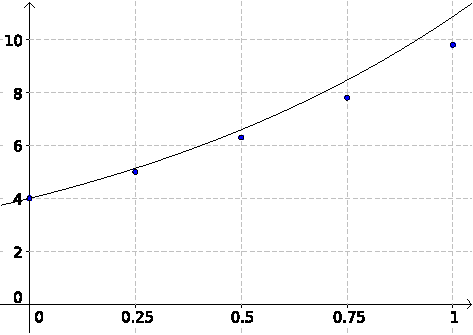
\includegraphics{figures/ode-pendulum03}
\par\end{center}
\item [{\ref{exc:odePendulum-17}:}] Dari grafik solusi eksak dan solusi
aproksimasi, hampiran tersebut tampak sangat baik pada $t=0$ dan
$t=2$, tetapi tidak terlalu akurat di antara keduanya. Lebih tepatnya,
galat relatif pada $t=0.5,\ 1,\ 1.5$ masing-masing sekitar $.124$,
$.097$, dan $.095$. Pada tiga dari lima titik, galat relatifnya
sebesar $9.5$\% atau lebih.

\begin{center}
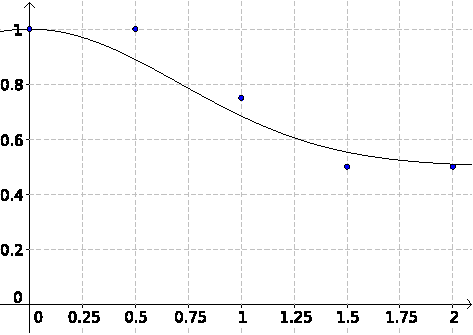
\includegraphics{figures/ode-pendulum04}
\par\end{center}
\item [{\ref{exc:odePendulum-19}:}] Dari grafik solusi eksak dan solusi
aproksimasi, hampiran tersebut tampak sangat baik untuk semua nilai
$t$. Galat terbesar tampaknya terjadi pada $t=11$ dan $t=13$. Untuk
mengetahui seberapa baik hampiran tersebut, galat absolut pada $t=11$
dan $t=13$ masing-masing sekitar $.0066$ dan $.0044$, berturut-turut.
Galat relatifnya masing-masing sekitar $.021$ dan $.0073$, berturut-turut.
Semuanya merupakan galat yang kecil.

\begin{center}
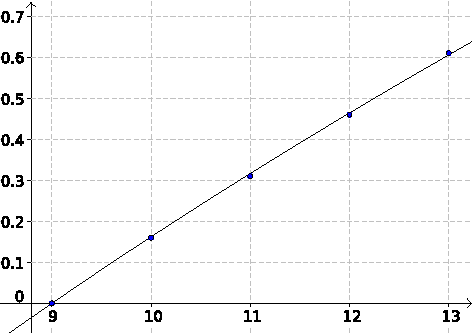
\includegraphics{figures/ode-pendulum05}
\par\end{center}
\item [{\ref{exc:odePendulum-20}:}]~

\begin{center}
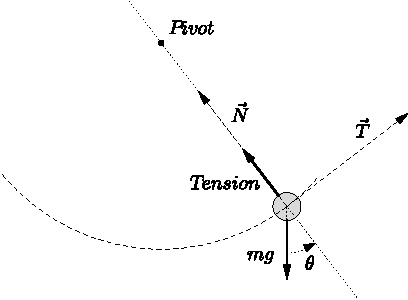
\includegraphics{figures/ode-pendulum06}
\par\end{center}
\item [{\ref{exc:odePendulum-21}:}]~

\begin{center}
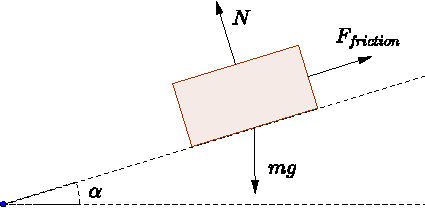
\includegraphics{figures/ode-pendulum07}
\par\end{center}
\item [{\ref{exc:odePendulum-23}:}] $F_{applied}$ dan $F_{friction}$
dapat dipertukarkan.

\begin{center}
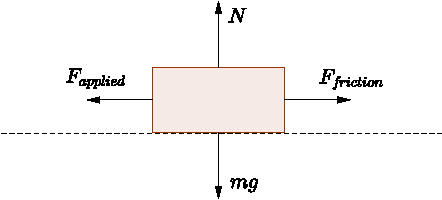
\includegraphics{figures/ode-pendulum08}
\par\end{center}
\item [{\ref{exc:odePendulum-25}:}]~

\begin{center}
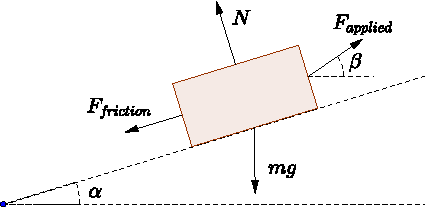
\includegraphics{figures/ode-pendulum09}
\par\end{center}
\item [{\ref{exc:odePendulum-26}:}]~

\begin{center}
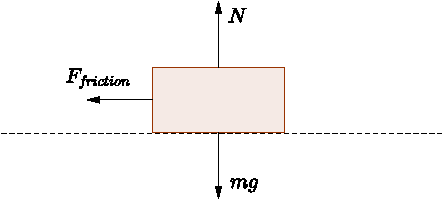
\includegraphics{figures/ode-pendulum10}
\par\end{center}
\item [{\ref{exc:odePendulum-27}:}]~

\begin{center}
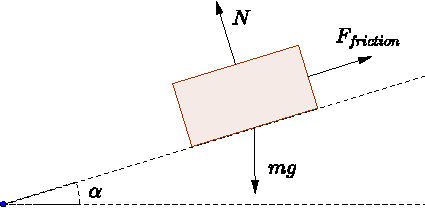
\includegraphics{figures/ode-pendulum07}
\par\end{center}
\item [{\ref{exc:odePendulum-28}:}]~

\begin{center}
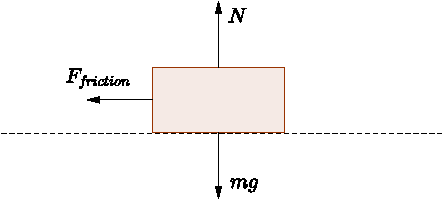
\includegraphics{figures/ode-pendulum10}
\par\end{center}
\item [{\ref{exc:odePendulum-29}:}]~

\begin{center}
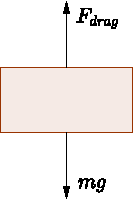
\includegraphics{figures/ode-pendulum11}
\par\end{center}
\item [{\ref{exc:odePendulum-31}:}]~

\begin{center}
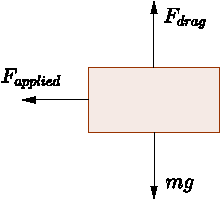
\includegraphics{figures/ode-pendulum12}
\par\end{center}
\item [{\ref{exc:odePendulum-32}:}]~

\begin{center}
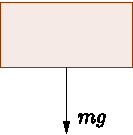
\includegraphics{figures/ode-pendulum13}
\par\end{center}
\item [{\ref{exc:odePendulum-34}:}] (\ref{exc:odePendulum-20}) $\ddot{\theta}+\frac{g}{\ell}\sin\theta=0$;
(\ref{exc:odePendulum-21}) dengan arah menuruni lereng sebagai arah
positif: $\ddot{s}=g(\sin\alpha-\mu\cos\alpha)$; (\ref{exc:odePendulum-23})
$\ddot{s}=\frac{1}{m}F_{applied}-\mu g$; (\ref{exc:odePendulum-25})
dengan arah mendaki lereng sebagai arah positif: $\ddot{s}=\frac{1}{m}F_{applied}\cos(\beta-\alpha)-g(\sin\alpha+\mu\cos\alpha)$;
(\ref{exc:odePendulum-26}) dengan arah gerak kereta luncur sebagai
arah positif: $\ddot{s}=-\mu g$; (\ref{exc:odePendulum-27}) dengan
arah menuruni lereng sebagai arah positif: $\ddot{s}=g(\sin\alpha-\mu\cos\alpha)$;
(\ref{exc:odePendulum-28}) dengan arah gerak keping hoki sebagai
arah positif: $\ddot{s}=-\mu g$; (\ref{exc:odePendulum-29}) dengan
arah ke atas sebagai arah positif: $\ddot{s}=\frac{c}{m}\dot{s}-g$;
(\ref{exc:odePendulum-31}) dengan arah ke atas sebagai arah positif:
$\ddot{s}=\frac{c}{m}\dot{s}-g$; (\ref{exc:odePendulum-32}) dengan
arah ke atas sebagai arah positif: $\ddot{s}=-g$
\item [{\ref{exc:odePendulum-33}:}] Gesekan kinetik: $\mu mg$ dibandingkan
dengan $\mu(mg+F_{applied}\sin20^{\circ})$. Gaya terapan yang diperlukan
untuk mengatasi gesekan: $\mu mg$ dibandingkan dengan $\frac{\mu mg}{\cos20^{\circ}-\mu\sin20^{\circ}}$.
Gaya terapan yang mendorong sejajar lantai hanya perlu sebesar $(\cos20^{\circ}-\mu\sin20^{\circ})$
kali gaya ketika mendorong dengan sudut $20^{\circ}$ dari arah sejajar.
Sebagai contoh, ketika $\mu=.3$, $\cos20^{\circ}-\mu\sin20^{\circ}\approx.837$
sehingga gaya yang diperlukan saat mendorong sejajar lantai hanya
83,7\% dari gaya yang diperlukan saat mendorong dengan sudut $20^{\circ}$
dari arah sejajar.
\end{description}

\section*{Bagian \ref{sec:TaylorMethods}}
\begin{description}
\item [{\ref{exc:ode-taylor-7}:}] $y(2)\approx1.3125$
\item [{\ref{exc:ode-taylor-9}c:}] $y(2)\approx1.88671875$
\item [{\ref{exc:ode-taylor-10}c:}] $y(2)\approx2.126953125$
\item [{\ref{exc:ode-taylor-1}:}] $y(1.5)\approx0.8203125$
\item [{\ref{exc:ode-taylor-11}:}] $\ $

\begin{pseudocode} \index{metode Taylor orde 2!kode semu}
\begin{description}
\item [{Asumsi:}] Solusi PDB ada dan tunggal pada selang dari $t_{0}$
hingga $t_{1}$.
\item [{Masukan:}] Persamaan diferensial $\dot{y}=f(t,y)$; rumus $\ddot{y}(t,y)$;
kondisi awal $y(t_{0})=y_{0}$; bilangan $t_{0}$ dan $t_{1}$; jumlah
langkah $N$.
\item [{Langkah\ 1:}] Tetapkan $t=t_{0}$; $y=y_{0}$; $h=(t_{1}-t_{0})/N$
\item [{Langkah~2:}] Untuk $j=1\ldots N$ lakukan Langkah 3--4:

\begin{description}
\item [{Langkah~3:}] Tetapkan $y=y+hf(t,y)+\frac{1}{2}h^{2}\ddot{y}(t,y)$
\item [{Langkah~4:}] Tetapkan $t=t_{0}+\frac{i}{N}(t_{1}-t_{0})$
\end{description}
\item [{Keluaran:}] Hampiran $y$ untuk solusi di $t=t_{1}$.
\end{description}
\end{pseudocode} 
\item [{\ref{exc:ode-taylor-3}:}] $\ $\index{metode Taylor orde 2!kode}
\texttt{taylor2ode.m} dapat diunduh dari \href{http://lqbrin.github.io/tea-time-numerical/ancillaries.html}{situs pendamping}.

\begin{lyxcode}
\%\%\%\%\%\%\%\%\%\%\%\%\%\%\%\%\%\%\%\%\%\%\%\%\%\%\%\%\%\%\%\%\%\%\%\%\%\%\%\%\%\%\%\%\%\%\%\%\%\%\%\%\%\%\%\%\%\%\%\%\%\%\%\%\%\%

\%~Written~by~Leon~Brin~~~~~~~~~~~~~~~~~~~~~~~~~~13~November~2015~\%

\%~Purpose:~This~function~implements~Taylor's~method~of~order~2~~~\%

\%~~~~~~~~where~the~step~size~is~calculated~and~held~constant.~~~~\%

\%~INPUT:~function~f(x,y);~function~(df/dx)(x,y);~interval~{[}a,b{]};~\%

\%~~~~~~~~y(a);~steps~n~~~~~~~~~~~~~~~~~~~~~~~~~~~~~~~~~~~~~~~~~~~\%

\%~OUTPUT:~approximation~(x(i),y(i))~of~the~solution~of~y'=f(x,y)~\%

\%\%\%\%\%\%\%\%\%\%\%\%\%\%\%\%\%\%\%\%\%\%\%\%\%\%\%\%\%\%\%\%\%\%\%\%\%\%\%\%\%\%\%\%\%\%\%\%\%\%\%\%\%\%\%\%\%\%\%\%\%\%\%\%\%\%

function~{[}y,x{]}~=~taylor2ode(f,ft,a,ya,b,n)

~~i~=~1;

~~x(i)~=~a;

~~y(i)~=~ya;

~~h~=~(b-a)/n;

~~while~(i<=n)

~~~~y(i+1)~=~y(i)~+~h{*}(f(x(i),y(i))~+~0.5{*}h{*}ft(x(i),y(i)));

~~~~x(i+1)~=~a~+~(b-a){*}i/n;

~~~~i~=~i+1;

~~end\%while

end\%function~
\end{lyxcode}
\item [{\ref{exc:ode-taylor-12}:}] 
\[
y(2)\approx2.3125,\,2.28814697265625,\,2.28469446951954,\,2.28402793464698
\]
 galat absolutnya kira-kira 
\[
0.02866617919084,\,0.004313151847096,\,8.606487103870(10)^{-4},\,1.941138378267(10)^{-4}
\]
 rasio galatnya kira-kira $6.6,\,5.0,\,4.4$.
\item [{\ref{exc:ode-taylor-13}a:}] 
\begin{eqnarray*}
\dot{u} & = & -\frac{g}{\ell}\sin\theta\\
\dot{\theta} & = & u
\end{eqnarray*}
\item [{\ref{exc:ode-taylor-13}b:}] 
\begin{eqnarray*}
\dot{u} & = & g(\sin\alpha-\mu\cos\alpha)\\
\dot{s} & = & u
\end{eqnarray*}
\item [{\ref{exc:ode-taylor-13}e:}] 
\begin{eqnarray*}
\dot{u} & = & \frac{1}{m}F_{applied}-\mu g\\
\dot{s} & = & u
\end{eqnarray*}
\item [{\ref{exc:ode-taylor-13}g:}] 
\begin{eqnarray*}
\dot{u} & = & \frac{1}{m}F_{applied}\cos(\beta-\alpha)-g(\sin\alpha+\mu\cos\alpha)\\
\dot{s} & = & u
\end{eqnarray*}
\item [{\ref{exc:ode-taylor-13}h:}] 
\begin{eqnarray*}
\dot{u} & = & -\mu g\\
\dot{s} & = & u
\end{eqnarray*}
\item [{\ref{exc:ode-taylor-13}i:}] 
\begin{eqnarray*}
\dot{u} & = & g(\sin\alpha-\mu\cos\alpha)\\
\dot{s} & = & u
\end{eqnarray*}
\item [{\ref{exc:ode-taylor-13}j:}] 
\begin{eqnarray*}
\dot{u} & = & -\mu g\\
\dot{s} & = & u
\end{eqnarray*}
\item [{\ref{exc:ode-taylor-13}l:}] 
\begin{eqnarray*}
\dot{u} & = & \frac{c}{m}u-g\\
\dot{s} & = & u
\end{eqnarray*}
\item [{\ref{exc:ode-taylor-21}:}] (a) $-0.6656470478206087$ (b) $0.2384138557742662$
(e) $0.05695982142857142$ (g) $0.2313498206324268$ (h) $14.979875$
(i) $5.988821238748838$ (j) $43.9939625$ (l) $4.387767857142857$
\item [{\ref{exc:ode-taylor-15}:}] $y(x)=\frac{3}{2}x-\frac{5}{4}$
\item [{\ref{exc:ode-taylor-16}:}] $y(x)=\frac{2}{7}x^{2}+\frac{11}{7}x+\frac{143}{49}$
\item [{\ref{exc:ode-taylor-17}:}] $y(t)=t^{4}-8t^{3}+48t^{2}-192t+385$
\item [{\ref{exc:ode-taylor-20}:}] $\theta(t)=-\frac{2}{5}e^{-t}\sin t-\frac{1}{5}e^{-t}\cos t$
\item [{\ref{exc:ode-taylor-19}:}] $x(t)=\frac{1}{12}te^{7t}-\frac{1}{35}$
\end{description}

\section*{Bagian \ref{sec:Runge-Kutta-Methods}}
\begin{description}
\item [{\ref{exc:ode-rungeKutta-2}:}] $\ $
\begin{eqnarray*}
k_{1} & = & f(t_{i},y_{i})\\
k_{2} & = & f\left(t_{i}+\frac{h}{2},y_{i}+\frac{h}{2}k_{1}\right)\\
y_{i+1} & = & y_{i}+hk_{2}
\end{eqnarray*}
\item [{\ref{exc:ode-rungeKutta-3}:}] $\ $
\begin{eqnarray*}
k_{1} & = & f(t_{i},y_{i})\\
k_{2} & = & f\left(t_{i}+\frac{h}{3},y_{i}+\frac{h}{3}k_{1}\right)\\
y_{i+1} & = & y_{i}+\frac{h}{2}\left[3k_{2}-k_{1}\right]
\end{eqnarray*}
\item [{\ref{exc:ode-rungeKutta-7}:}] $\ $
\begin{eqnarray*}
k_{1} & = & f(t_{i},y_{i})\\
k_{2} & = & f\left(t_{i}+\frac{h}{3},y_{i}+\frac{h}{3}k_{1}\right)\\
k_{3} & = & f\left(t_{i}+\frac{h}{2},y_{i}+\frac{h}{2}k_{2}\right)\\
k_{4} & = & f\left(t_{i}+\frac{2h}{3},y_{i}+\frac{2h}{3}k_{1}\right)\\
y_{i+1} & = & y_{i}+\frac{h}{2}\left[3k_{2}-4k_{3}+3k_{4}\right]
\end{eqnarray*}
\item [{\ref{exc:ode-rungeKutta-10}:}] $\ $
\begin{eqnarray*}
k_{1} & = & f(t_{i},y_{i})\\
k_{2} & = & f\left(t_{i}+\frac{\sqrt{5}-\sqrt{3}}{2\sqrt{5}}h,y_{i}+\frac{\sqrt{5}-\sqrt{3}}{2\sqrt{5}}hk_{1}\right)\\
k_{3} & = & f\left(t_{i}+\frac{h}{2},y_{i}+\frac{h}{2}k_{2}\right)\\
k_{4} & = & f\left(t_{i}+\frac{\sqrt{5}+\sqrt{3}}{2\sqrt{5}}h,y_{i}+\frac{\sqrt{5}+\sqrt{3}}{2\sqrt{5}}hk_{1}\right)\\
y_{i+1} & = & y_{i}+\frac{h}{18}\left[5k_{2}+8k_{3}+5k_{4}\right]
\end{eqnarray*}
\item [{\ref{exc:ode-rungeKutta-16}b:}] $O(h^{2})$; Ya
\item [{\ref{exc:ode-rungeKutta-16}c:}] $O(h^{2})$; Ya
\item [{\ref{exc:ode-rungeKutta-16}g:}] $O(h^{3})$; Tidak
\item [{\ref{exc:ode-rungeKutta-16}j:}] $O(h^{2})$; Tidak
\item [{\ref{exc:ode-rungeKutta-14}:}] \vpageref{code:euler}
\item [{\ref{exc:ode-rungeKutta-11}:}] $\ $\index{metode titik tengah!kode}
\end{description}
\begin{lyxcode}
\%\%\%\%\%\%\%\%\%\%\%\%\%\%\%\%\%\%\%\%\%\%\%\%\%\%\%\%\%\%\%\%\%\%\%\%\%\%\%\%\%\%\%\%\%\%\%\%\%\%\%\%\%\%\%\%\%\%\%\%\%\%\%\%\%\%

\%~Written~by~Leon~Brin~~~~~~~~~~~~~~~~~~~~~~~~~~~~~~~28~May~2016~\%

\%~Purpose:~This~function~implements~the~Midpoint~method~where~~~~\%

\%~~~~~~~~the~step~size~is~calculated~and~held~constant.~~~~~~~~~~\%

\%~INPUT:~function~f(x,y);~interval~{[}a,b{]};~y(a);~steps~n~~~~~~~~~~\%

\%~OUTPUT:~approximation~(x(i),y(i))~of~the~solution~of~y'=f(x,y)~\%

\%\%\%\%\%\%\%\%\%\%\%\%\%\%\%\%\%\%\%\%\%\%\%\%\%\%\%\%\%\%\%\%\%\%\%\%\%\%\%\%\%\%\%\%\%\%\%\%\%\%\%\%\%\%\%\%\%\%\%\%\%\%\%\%\%\%

function~{[}y,x{]}~=~midpoint(f,a,ya,b,n)

~~i~=~1;

~~x(i)~=~a;

~~y(i)~=~ya;

~~h~=~(b-a)/n;

~~while~(i<=n)

~~~~k1~=~f(x(i),y(i));

~~~~k2~=~f(x(i)+h/2,y(i)+h/2{*}k1);

~~~~y(i+1)~=~y(i)~+~h{*}k2;

~~~~x(i+1)~=~a~+~(b-a){*}i/n;

~~~~i~=~i+1;

~~end\%while

end\%function~

\textrm{Kode ini dapat diunduh dari \href{http://lqbrin.github.io/tea-time-numerical/ancillaries.html}{situs pendamping}.}
\end{lyxcode}
\begin{description}
\item [{\ref{exc:ode-rungeKutta-15}:}] $\ $\index{metode Ralston!kode}
\end{description}
\begin{lyxcode}
\%\%\%\%\%\%\%\%\%\%\%\%\%\%\%\%\%\%\%\%\%\%\%\%\%\%\%\%\%\%\%\%\%\%\%\%\%\%\%\%\%\%\%\%\%\%\%\%\%\%\%\%\%\%\%\%\%\%\%\%\%\%\%\%\%\%

\%~Written~by~Leon~Brin~~~~~~~~~~~~~~~~~~~~~~~~~~~~~~~28~May~2016~\%

\%~Purpose:~This~function~implements~Ralston's~method~where~~~~~~~\%

\%~~~~~~~~the~step~size~is~calculated~and~held~constant.~~~~~~~~~~\%

\%~INPUT:~function~f(x,y);~interval~{[}a,b{]};~y(a);~steps~n~~~~~~~~~~\%

\%~OUTPUT:~approximation~(x(i),y(i))~of~the~solution~of~y'=f(x,y)~\%

\%\%\%\%\%\%\%\%\%\%\%\%\%\%\%\%\%\%\%\%\%\%\%\%\%\%\%\%\%\%\%\%\%\%\%\%\%\%\%\%\%\%\%\%\%\%\%\%\%\%\%\%\%\%\%\%\%\%\%\%\%\%\%\%\%\%

function~{[}y,x{]}~=~ralston(f,a,ya,b,n)

~~i~=~1;

~~x(i)~=~a;

~~y(i)~=~ya;

~~h~=~(b-a)/n;

~~while~(i<=n)

~~~~k1~=~f(x(i),y(i));

~~~~k2~=~f(x(i)+2{*}h/3,y(i)+2{*}h/3{*}k1);

~~~~y(i+1)~=~y(i)~+~h/4{*}(k1+3{*}k2);

~~~~x(i+1)~=~a~+~(b-a){*}i/n;

~~~~i~=~i+1;

~~end\%while

end\%function~

\textrm{Kode ini dapat diunduh dari \href{http://lqbrin.github.io/tea-time-numerical/ancillaries.html}{situs pendamping}.}
\end{lyxcode}
\begin{description}
\item [{\ref{exc:ode-rungeKutta-17}c:}] $2.071336302192492$
\item [{\ref{exc:ode-rungeKutta-18}c:}] $2.237523715781341$
\item [{\ref{exc:ode-rungeKutta-19}c:}] $2.240722979472185$
\item [{\ref{exc:ode-rungeKutta-20}c:}] $2.235615854209425$
\item [{\ref{exc:ode-rungeKutta-21}c:}] $2.236251636584492$
\end{description}

\section*{Bagian \ref{sec:Runge-Kutta-Error-Analysis}}
\begin{description}
\item [{\ref{exc:ode-errorAnalysis}b:}] $O(h^{3})$; sama dengan galat
pemenggalan lokal rumus integrasi yang mendasarinya; ya, satu derajat
lebih tinggi daripada laju kekonvergenan.
\item [{\ref{exc:ode-errorAnalysis}c:}] $O(h^{3})$; sama dengan galat
pemenggalan lokal rumus integrasi yang mendasarinya; ya, satu derajat
lebih tinggi daripada laju kekonvergenan.
\item [{\ref{exc:ode-errorAnalysis}g:}] CATATAN: Karena ini merupakan
metode empat tahap, persamaan \ref{eq:rk4cond1}-\ref{eq:rk4cond10}
harus digunakan untuk menentukan laju kekonvergenan. $O(h^{4})$;
lebih rendah daripada galat pemenggalan lokal rumus integrasi yang
mendasarinya; ya, satu derajat lebih tinggi daripada laju kekonvergenan.
\item [{\ref{exc:ode-errorAnalysis}j:}] CATATAN: Karena ini merupakan
metode empat tahap, persamaan \ref{eq:rk4cond1}-\ref{eq:rk4cond10}
harus digunakan untuk menentukan laju kekonvergenan. $O(h^{3})$;
lebih rendah daripada galat pemenggalan lokal rumus integrasi yang
mendasarinya; ya, satu derajat lebih tinggi daripada laju kekonvergenan.
\item [{\ref{exc:ode-errorAnalysis-2}:}] $\ $\index{metode Euler yang diperbaiki!kode}
\texttt{eulerimp.m} dapat diunduh dari \href{http://lqbrin.github.io/tea-time-numerical/ancillaries.html}{situs pendamping}.

\begin{lyxcode}
\%\%\%\%\%\%\%\%\%\%\%\%\%\%\%\%\%\%\%\%\%\%\%\%\%\%\%\%\%\%\%\%\%\%\%\%\%\%\%\%\%\%\%\%\%\%\%\%\%\%\%\%\%\%\%\%\%\%\%\%\%\%\%\%\%\%

\%~Written~by~Leon~Brin~~~~~~~~~~~~~~~~~~~~~~~~~~~~~~~31~May~2016~\%

\%~Purpose:~This~function~implements~improved~Euler's~method~~~~~~\%

\%~~~~~~~~where~the~step~size~is~calculated~and~held~constant.~~~~\%

\%~INPUT:~function~f(x,y);~interval~{[}a,b{]};~y(a);~steps~n~~~~~~~~~~\%

\%~OUTPUT:~approximation~(x(i),y(i))~of~the~solution~of~y'=f(x,y)~\%

\%\%\%\%\%\%\%\%\%\%\%\%\%\%\%\%\%\%\%\%\%\%\%\%\%\%\%\%\%\%\%\%\%\%\%\%\%\%\%\%\%\%\%\%\%\%\%\%\%\%\%\%\%\%\%\%\%\%\%\%\%\%\%\%\%\%

function~{[}y,x{]}~=~eulerimp(f,a,ya,b,n)

~~i~=~1;

~~x(i)~=~a;

~~y(i)~=~ya;

~~h~=~(b-a)/n;

~~while~(i<=n)

~~~~k1~=~f(x(i),y(i));

~~~~k2~=~f(x(i)+h,y(i)~+~h{*}k1);

~~~~y(i+1)~=~y(i)~+~h/2{*}(k1+k2);

~~~~x(i+1)~=~a~+~(b-a){*}i/n;

~~~~i~=~i+1;

~~end\%while

end\%function
\end{lyxcode}
\item [{\ref{exc:ode-errorAnalysis-3}:}] $\ $\index{metode orde ketiga Heun!kode}
\texttt{heun.m} dapat diunduh dari \href{http://lqbrin.github.io/tea-time-numerical/ancillaries.html}{situs pendamping}.

\begin{lyxcode}
\%\%\%\%\%\%\%\%\%\%\%\%\%\%\%\%\%\%\%\%\%\%\%\%\%\%\%\%\%\%\%\%\%\%\%\%\%\%\%\%\%\%\%\%\%\%\%\%\%\%\%\%\%\%\%\%\%\%\%\%\%\%\%\%\%\%

\%~Written~by~Leon~Brin~~~~~~~~~~~~~~~~~~~~~~~~~~~~~~~31~May~2016~\%

\%~Purpose:~This~function~implements~Heun's~third~order~method~~~~\%

\%~~~~~~~~where~the~step~size~is~calculated~and~held~constant.~~~~\%

\%~INPUT:~function~f(x,y);~interval~{[}a,b{]};~y(a);~steps~n~~~~~~~~~~\%

\%~OUTPUT:~approximation~(x(i),y(i))~of~the~solution~of~y'=f(x,y)~\%

\%\%\%\%\%\%\%\%\%\%\%\%\%\%\%\%\%\%\%\%\%\%\%\%\%\%\%\%\%\%\%\%\%\%\%\%\%\%\%\%\%\%\%\%\%\%\%\%\%\%\%\%\%\%\%\%\%\%\%\%\%\%\%\%\%\%

function~{[}y,x{]}~=~heun(f,a,ya,b,n)

~~i~=~1;

~~x(i)~=~a;

~~y(i)~=~ya;

~~h~=~(b-a)/n;

~~while~(i<=n)

~~~~k1~=~f(x(i),~y(i));

~~~~k2~=~f(x(i)+h/3,~y(i)+h/3{*}k1);

~~~~k3~=~f(x(i)+2{*}h/3,~y(i)+2{*}h/3{*}k2);

~~~~y(i+1)~=~y(i)~+~h/4{*}(k1+3{*}k3);

~~~~x(i+1)~=~a~+~(b-a){*}i/n;

~~~~i~=~i+1;

~~end\%while

end\%function
\end{lyxcode}
\item [{\ref{exc:ode-errorAnalysis-4}:}] \index{metode RK4!kode}\texttt{
rk4.m} dapat diunduh dari \href{http://lqbrin.github.io/tea-time-numerical/ancillaries.html}{situs pendamping}.

\begin{lyxcode}
\%\%\%\%\%\%\%\%\%\%\%\%\%\%\%\%\%\%\%\%\%\%\%\%\%\%\%\%\%\%\%\%\%\%\%\%\%\%\%\%\%\%\%\%\%\%\%\%\%\%\%\%\%\%\%\%\%\%\%\%\%\%\%\%\%\%

\%~Written~by~Leon~Brin~~~~~~~~~~~~~~~~~~~~~~~~~~~~~~~1~June~2016~\%

\%~Purpose:~This~function~implements~Runge-Kutta~4th~order~(RK4)~~\%

\%~~~~~~~~where~the~step~size~is~calculated~and~held~constant.~~~~\%

\%~INPUT:~function~f(x,y);~interval~{[}a,b{]};~y(a);~steps~n~~~~~~~~~~\%

\%~OUTPUT:~approximation~(x(i),y(i))~of~the~solution~of~y'=f(x,y)~\%

\%\%\%\%\%\%\%\%\%\%\%\%\%\%\%\%\%\%\%\%\%\%\%\%\%\%\%\%\%\%\%\%\%\%\%\%\%\%\%\%\%\%\%\%\%\%\%\%\%\%\%\%\%\%\%\%\%\%\%\%\%\%\%\%\%\%

function~{[}y,x{]}~=~rk4(f,a,ya,b,n)

~~i~=~1;

~~x(i)~=~a;

~~y(i)~=~ya;

~~h~=~(b-a)/n;

~~while~(i<=n)

~~~~k1~=~f(x(i),~y(i));

~~~~k2~=~f(x(i)+h/2,~y(i)+h/2{*}k1);

~~~~k3~=~f(x(i)+h/2,~y(i)+h/2{*}k2);

~~~~k4~=~f(x(i)+h,~y(i)+h{*}k3);

~~~~y(i+1)~=~y(i)~+~h/6{*}(k1+2{*}k2+2{*}k3+k4);

~~~~x(i+1)~=~a~+~(b-a){*}i/n;

~~~~i~=~i+1;

~~end\%while

end\%function
\end{lyxcode}
\end{description}

\section*{Bagian \ref{sec:Adaptive-Runge-Kutta-Methods}}
\begin{description}
\item [{\ref{exc:ode-adaptive}:}] Salah satu cara mengodekannya adalah
sebagai berikut.\index{metode RK2(3)!kode} \texttt{rk23.m} dapat
diunduh dari \href{http://lqbrin.github.io/tea-time-numerical/ancillaries.html}{situs pendamping}.

\begin{lyxcode}
\%\%\%\%\%\%\%\%\%\%\%\%\%\%\%\%\%\%\%\%\%\%\%\%\%\%\%\%\%\%\%\%\%\%\%\%\%\%\%\%\%\%\%\%\%\%\%\%\%\%\%\%\%\%\%\%\%\%\%\%\%\%\%\%\%\%

\%~Written~by~Leon~Brin~~~~~~~~~~~~~~~~~~~~~~~~~~~~~~~31~May~2016~\%

\%~Purpose:~This~function~implements~an~adaptive~rk2(3)~method~~~~\%

\%~~~~~~~~where~the~step~size~is~controlled~by~the~routine.~~~~~~~\%

\%~~~~~~~~Heun's~third~order~method~is~combined~with~open-ode.~~~~\%

\%~INPUT:~function~f(x,y);~interval~{[}a,b{]};~y(a);~initial~step~~~~~\%

\%~~~~~~~~size~h;~tolerance~eps;~maximum~steps~N;~~~~~~~~~~~~~~~~~\%

\%~OUTPUT:~approximation~(x(i),y(i))~of~the~solution~of~y'=f(x,y)~\%

\%\%\%\%\%\%\%\%\%\%\%\%\%\%\%\%\%\%\%\%\%\%\%\%\%\%\%\%\%\%\%\%\%\%\%\%\%\%\%\%\%\%\%\%\%\%\%\%\%\%\%\%\%\%\%\%\%\%\%\%\%\%\%\%\%\%

function~{[}y,t{]}~=~rk23(f,a,ya,b,h,eps,N)

~~i~=~1;

~~t(i)~=~a;

~~y(i)~=~ya;

~~done~=~0;

~~while~(!done~\&\&~i<=N)

~~~~if~((b-t(i)-h){*}(b-a)<=0)

~~~~~~h=b-t(i);

~~~~~~done~=~1;

~~~~endif

~~~~k1~=~f(t(i),~y(i));

~~~~k2~=~f(t(i)+h/3,~y(i)+h/3{*}k1);

~~~~k3~=~f(t(i)+2{*}h/3,~y(i)+2{*}h/3{*}k2);

~~~~err~=~abs(h/4{*}(k1-2{*}k2+k3));

~~~~if~(done~||~err<=eps)

~~~~~~y(i+1)~=~y(i)~+~h/4{*}(k1+3{*}k3);

~~~~~~t(i+1)~=~t(i)~+~h;

~~~~~~if~(t(i+1)~==~t(i))

~~~~~~~~disp(\textquotedbl Procedure~failed.~Step~size~reached~zero.\textquotedbl )

~~~~~~~~return

~~~~~~endif

~~~~~~i~=~i+1;

~~~~endif

~~~~q~=~0.9{*}realpow(eps/err,1/3);

~~~~q~=~max(q,0.1);

~~~~q~=~min(5.0,q);

~~~~h~=~q{*}h;

~~end\%while

~~if~(!done)

~~~~disp(\textquotedbl Procedure~failed.~Maximum~number~of~iterations~reached.\textquotedbl )

~~endif

end\%function
\end{lyxcode}
\item [{\ref{exc:ode-adaptive-6}:}] (a) dan (d).
\item [{\ref{exc:ode-adaptive-17}:}] Tableau Butcher-nya adalah

\begin{center}
\begin{tabular}{c|cccc}
0 &  &  &  & \tabularnewline
$\frac{1}{3}$ & $\frac{1}{3}$ &  &  & \tabularnewline
$\frac{2}{3}$ & $-\frac{1}{3}$ & $1$ &  & \tabularnewline
1 & $1$ & $-1$ & $1$ & \tabularnewline
\hline 
 & $\frac{1}{8}$ & $\frac{3}{8}$ & $\frac{3}{8}$ & $\frac{1}{8}$\tabularnewline
\hline 
 & $0$ & $\frac{1}{2}$ & $\frac{1}{2}$ & $0$\tabularnewline
\end{tabular}
\par\end{center}
\item [{\ref{exc:ode-adaptive-15}:}] Salah satu cara mengodekannya adalah
sebagai berikut.\index{metode Merson!kode} \texttt{merson.m} dapat
diunduh dari \href{http://lqbrin.github.io/tea-time-numerical/ancillaries.html}{situs pendamping}.

\begin{lyxcode}
\%\%\%\%\%\%\%\%\%\%\%\%\%\%\%\%\%\%\%\%\%\%\%\%\%\%\%\%\%\%\%\%\%\%\%\%\%\%\%\%\%\%\%\%\%\%\%\%\%\%\%\%\%\%\%\%\%\%\%\%\%\%\%\%\%\%

\%~Written~by~Leon~Brin~~~~~~~~~~~~~~~~~~~~~~~~~~~~~~~9~June~2016~\%

\%~Purpose:~This~function~implements~the~method~of~Merson~(1957)~~\%

\%~~~~~~~~where~the~step~size~is~controlled~by~the~routine.~~~~~~~\%

\%~INPUT:~function~f(x,y);~interval~{[}a,b{]};~y(a);~initial~step~~~~~\%

\%~~~~~~~~size~h;~tolerance~eps;~maximum~steps~N;~~~~~~~~~~~~~~~~~\%

\%~OUTPUT:~approximation~(x(i),y(i))~of~the~solution~of~y'=f(x,y)~\%

\%\%\%\%\%\%\%\%\%\%\%\%\%\%\%\%\%\%\%\%\%\%\%\%\%\%\%\%\%\%\%\%\%\%\%\%\%\%\%\%\%\%\%\%\%\%\%\%\%\%\%\%\%\%\%\%\%\%\%\%\%\%\%\%\%\%

function~{[}y,t{]}~=~merson(f,a,ya,b,h,eps,N)

~~i~=~1;

~~t(i)~=~a;

~~y(i)~=~ya;

~~done~=~0;

~~while~(!done~\&\&~i<=N)

~~~~if~((b-t(i)-h){*}(b-a)<=0)

~~~~~~h=b-t(i);

~~~~~~done~=~1;

~~~~endif

~~~~k1~=~f(t(i),~y(i));

~~~~k2~=~f(t(i)+h/3,~y(i)+h/3{*}k1);

~~~~k3~=~f(t(i)+h/3,~y(i)+h/6{*}(k1+k2));

~~~~k4~=~f(t(i)+h/2,~y(i)+h/8{*}(k1+3{*}k3));

~~~~k5~=~f(t(i)+h,~y(i)+h/2{*}(k1-3{*}k3+4{*}k4));

~~~~err~=~abs(h/30{*}(2{*}k1-9{*}k3+8{*}k4-k5));

~~~~if~(done~||~err<=eps)

~~~~~~y(i+1)~=~y(i)~+~h/6{*}(k1+4{*}k4+k5);

~~~~~~t(i+1)~=~t(i)~+~h;

~~~~~~if~(t(i+1)~==~t(i))

~~~~~~~~disp(\textquotedbl Procedure~failed.~Step~size~reached~zero.\textquotedbl )

~~~~~~~~return

~~~~~~endif

~~~~~~i~=~i+1;

~~~~endif

~~~~q~=~0.9{*}realpow(eps/err,1/4);

~~~~q~=~max(q,0.1);

~~~~q~=~min(5.0,q);

~~~~h~=~q{*}h;

~~end\%while

~~if~(!done)

~~~~disp(\textquotedbl Procedure~failed.~Maximum~number~of~iterations~reached.\textquotedbl )

~~endif

end\%function
\end{lyxcode}
\item [{\ref{exc:ode-adaptive-26}:}] Seperti terlihat pada diagram, sebagian
besar toleransi yang lebih besar daripada $10^{-4}$ tidak menghasilkan
galat global sebesar $10^{-4}$ atau kurang, meskipun ada pengecualian.
Jika sekadar menebak dan memeriksa, kemungkinan Anda akan memperoleh
toleransi sebesar $5(10)^{-5}$ atau kurang.

\begin{center}
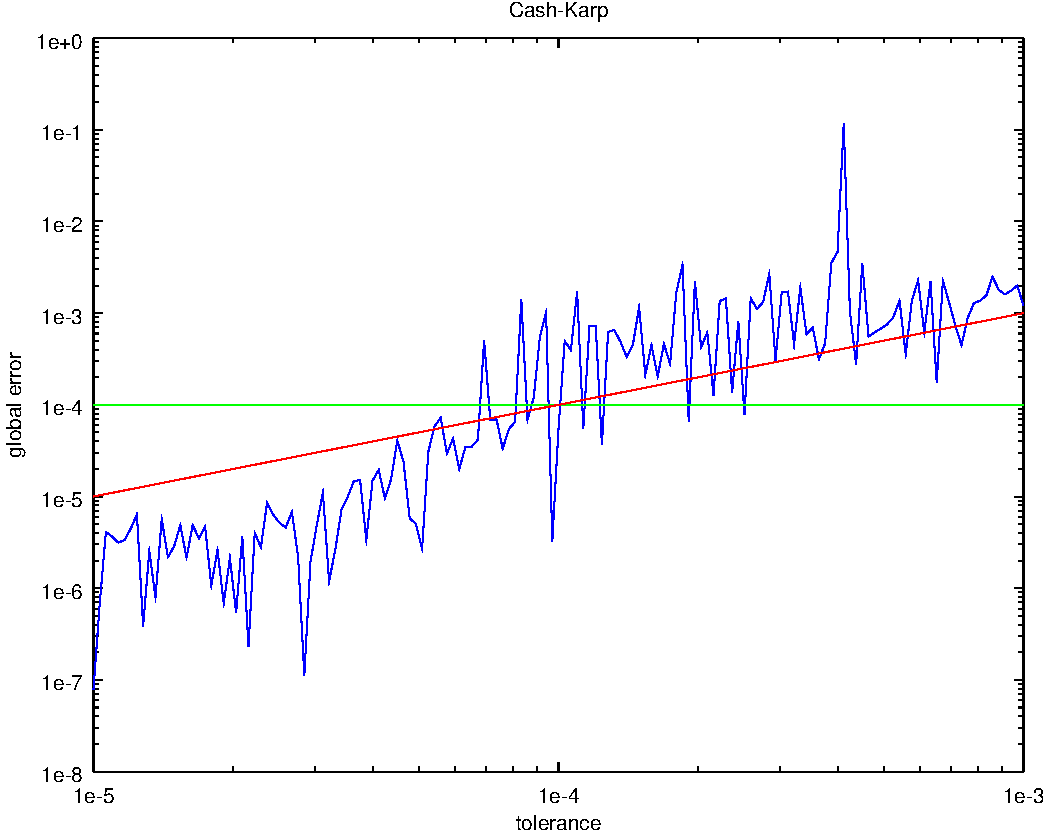
\includegraphics[scale=0.75]{figures/cashKarpGlobalError}
\par\end{center}
\item [{\ref{exc:ode-adaptive-27}:}] Seperti terlihat pada diagram, sebagian
besar toleransi yang lebih kecil daripada $10^{-3}$ menghasilkan
galat global sebesar $10^{-4}$ atau kurang, demikian pula beberapa
toleransi yang lebih besar.

\begin{center}
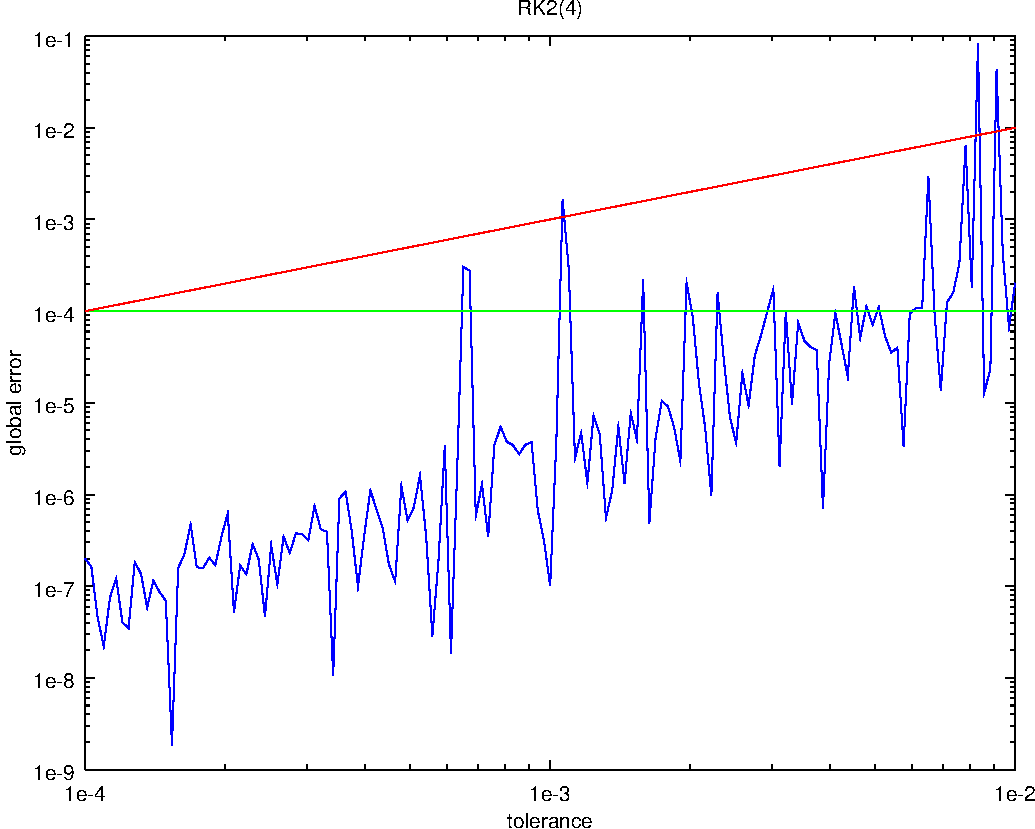
\includegraphics[scale=0.75]{figures/rk24globalError}
\par\end{center}
\item [{\ref{exc:ode-adaptive-29}:}] Seperti terlihat pada diagram, toleransi
yang lebih kecil daripada $10^{-4}$ menghasilkan galat global sebesar
$10^{-4}$ atau kurang, demikian pula beberapa toleransi yang sedikit
lebih tinggi.

\begin{center}
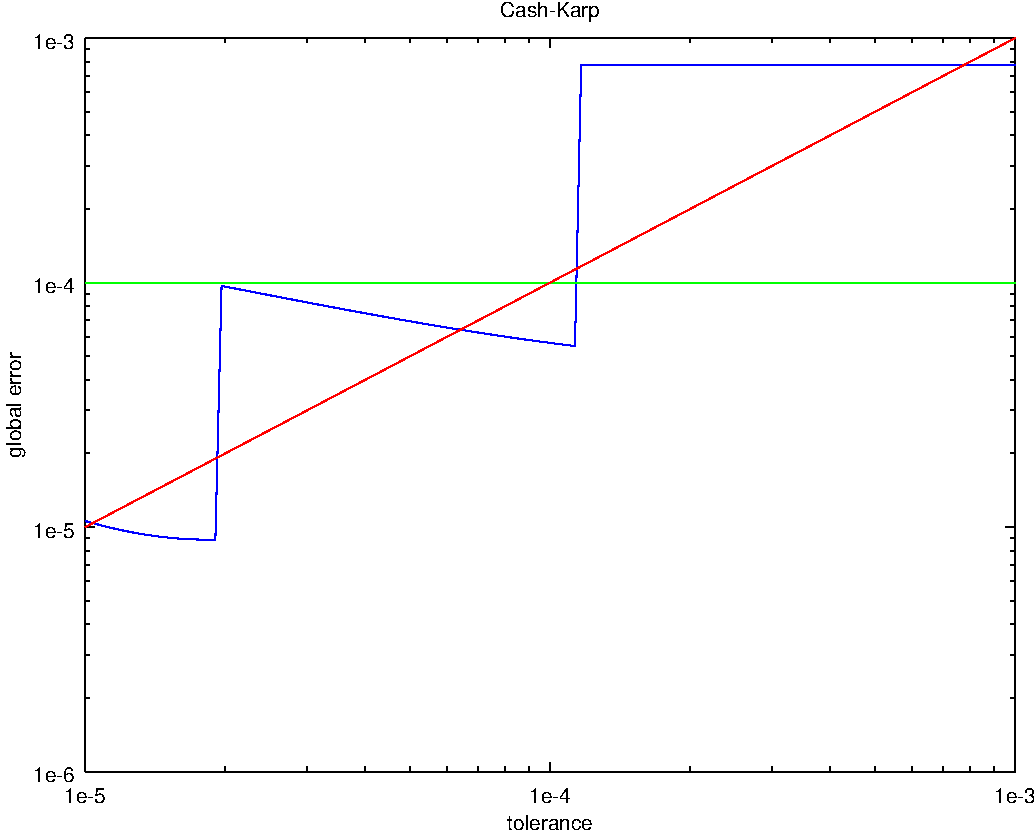
\includegraphics[scale=0.75]{figures/cashKarpGlobalError2}
\par\end{center}
\item [{\ref{exc:ode-adaptive-30}:}] Seperti terlihat pada diagram, sebagian
besar toleransi yang lebih kecil daripada sekitar $5(10)^{-3}$ menghasilkan
galat global sebesar $10^{-4}$ atau kurang, demikian pula beberapa
toleransi yang sedikit lebih besar.

\begin{center}
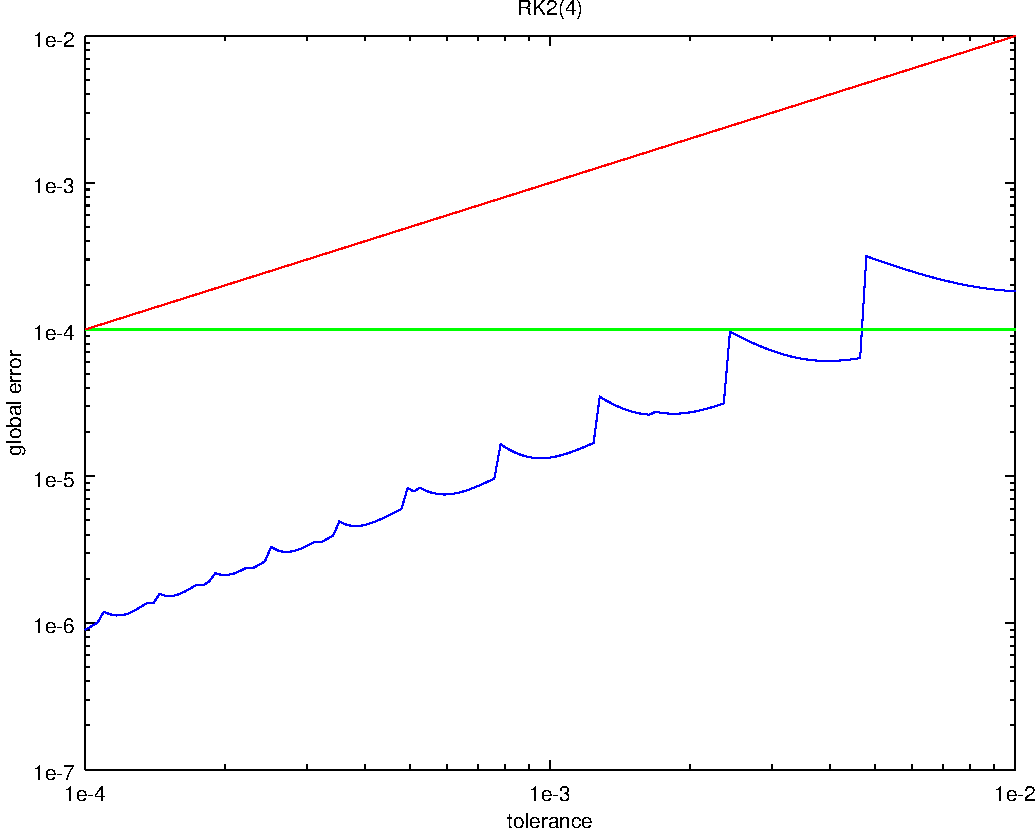
\includegraphics[scale=0.75]{figures/rk24globalError2}
\par\end{center}
\item [{\ref{exc:ode-adaptive-24}:}] (a) $y(5)\approx6.40926980783945$;
$\mbox{galat}\approx1.75(10)^{-4}$, 75\% lebih besar daripada toleransi.
(b) $y(5)\approx6.40708478227220$; $\mbox{galat}\approx2.36(10)^{-3}$,
hampir 24 kali toleransi. (c) $y(5)\approx6.40937679658180$; $\mbox{galat}\approx6.82(10)^{-5}$,
sekitar 68\% dari toleransi. (d) $y(5)\approx6.40885618182156$; $\mbox{galat}\approx5.88(10)^{-4}$,
hampir 6 kali toleransi.
\item [{\ref{exc:ode-adaptive-33}:}] Urutan dari yang paling efisien hingga
yang paling tidak efisien: Cash-Karp, Merson, RK2(3), Bogacki--Shampine,
masing-masing dengan 42, 50, 69, dan 138 penghitungan nilai fungsi.
\end{description}

